% !TEX TS-program = xelatex
% !TEX encoding = UTF-8
% !Mode:: "TeX:UTF-8"

\documentclass[onecolumn, oneside, ctexart]{SUSTechHomework}
\setlength{\parindent}{2em}
\linespread{1.5}
\usepackage{karnaugh-map}
\usepackage{float}
\usepackage{multicol}
\usepackage{tikz}
\usepackage{multirow}
\usetikzlibrary{arrows,automata,positioning}
\usepackage{longtable}
\usepackage{circuitikz}
\ctikzset{logic ports=ieee}
\usetikzlibrary{calc}

\coursecode{CS207}
\coursename{Digital Logic}
\title{Assignment 4}
\date{Dec. 22, 2021}

\lstset{language=verilog}

\begin{document}
  \maketitle
\section{DIGITAL DESIGN THEORY}

\subsection*{Q. 1}
\vspace{-2em}
\begin{longtable}[c]{cc|c}
\hline
J & K & Q(t+1) \\ \hline
\endfirsthead
%
\endhead
%
\hline
\endfoot
%
\endlastfoot
%
0 & 0 & Q      \\
0 & 1 & 0      \\
1 & 0 & 1      \\
1 & 1 & Q'     \\ \hline
\end{longtable}
\vspace{-1em}
\centerline{$Q_{t+1}=JQ'+K'Q$}
\vspace{1em}
\begin{longtable}[c]{c|c}
\hline
T & Q(t+1) \\ \hline
\endfirsthead
%
\endhead
%
0 & Q      \\
1 & Q'     \\ \hline 
\end{longtable}
\vspace{-1em}
\centerline{$Q_{t+1}=T'Q+TQ'=T\oplus Q$}

\subsection*{Q. 2}
\subsubsection*{(a)}
\vspace{-5em}
\begin{align*}
A(t+1)&=x'A'+B'A\\
B(t+1)&=xB'+AB
\end{align*}
\vspace{-4em}
\subsubsection*{(b)}
\begin{center}
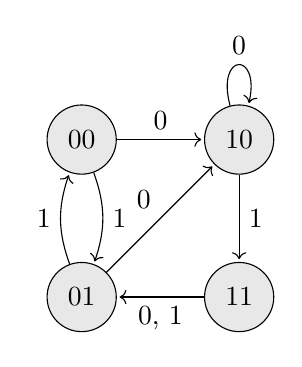
\begin{tikzpicture}[shorten >=1pt,node distance=2cm,auto]
  \tikzstyle{every state}=[fill={rgb:black,1;white,10}]

  \node[state] (zz)               {$00$};
  \node[state] (zo) [below of=zz] {$01$};
  \node[state] (oz) [right of=zz] {$10$};
  \node[state] (oo) [below of=oz] {$11$};

  \path[->]
  (zz)  edge [bend left=20] node {1} (zo)
        edge node {0} (oz)
  (zo)  edge [bend left=20] node {1} (zz)
        edge node {0} (oz)
  (oz)  edge [loop above] node {0} ( )
        edge node {1} (oo)
  (oo)  edge node {0, 1} (zo);
\end{tikzpicture}
\end{center}


\subsection*{Q. 3}
\vspace{-2em}
\begin{longtable}[c]{ccc|ccc|ccc}
\hline
\multicolumn{3}{c|}{Present State} & \multicolumn{3}{c|}{Next State}   & \multicolumn{3}{c}{Flip-Flop Inputs} \\ \hline
\endfirsthead
%
\endhead
%
\hline
\endfoot
%
\endlastfoot
%
$C_{t}$    & $B_{t}$   & $A_{t}$   & $C_{t+1}$ & $B_{t+1}$ & $A_{t+1}$ & $T_C$      & $T_B$      & $T_A$      \\ \hline
0          & 0         & 0         & 1         & 0         & 0         & 1          & 0          & 0          \\
0          & 0         & 1         & 0         & 0         & 0         & 0          & 0          & 1          \\
0          & 1         & 0         & X         & X         & X         & X          & X          & X          \\
0          & 1         & 1         & 0         & 0         & 1         & 0          & 1          & 0          \\
1          & 0         & 0         & 1         & 1         & 0         & 0          & 1          & 0          \\
1          & 0         & 1         & X         & X         & X         & X          & X          & X          \\
1          & 1         & 0         & 1         & 1         & 1         & 0          & 0          & 1          \\
1          & 1         & 1         & 0         & 1         & 1         & 1          & 0          & 0          \\ \hline
\end{longtable}
\vspace{-1em}
\par First by listing the state table (with don't care conditions) above, we can simplify the input equation:
\begin{align*}
T_A&=A\oplus B\\
T_B&=B\oplus C\\
T_C&=(A\oplus C)'
\end{align*}
\centerline{\includegraphics[width=0.35\textwidth]{fig/q31}}

\par One must notice that once the counter enters one of the unused states (a.k.a. 101 or 010) accidentally, the timing circuit will cycle through invalid states and will not be able to jump back to the scheduled state transfer sequence.
\begin{longtable}[c]{ccc|ccc|ccc}
\hline
\multicolumn{3}{c|}{Present State} & \multicolumn{3}{c|}{Flip-Flop Inputs} & \multicolumn{3}{c}{Next State}    \\ \hline
\endfirsthead
%
\endhead
%
$C_{t}$    & $B_{t}$   & $A_{t}$   & $T_C$       & $T_B$      & $T_A$      & $C_{t+1}$ & $B_{t+1}$ & $A_{t+1}$ \\ \hline
0          & 1         & 0         & 1           & 1          & 1          & 1         & 0         & 1         \\
1          & 0         & 1         & 1           & 1          & 1          & 0         & 1         & 0        \\ \hline
\end{longtable}

\par To avoid this, we should change our design to let the FSM that enters the unused state enter one of the valid states at the next clock pulse.
\par We can simply change $T_C=(A\oplus C)'$ to $T_C=ABC+A'B'C'$, then the FSM can correct these two unused states as shown below.

\pagebreak

\begin{multicols}{2}

\begin{center}
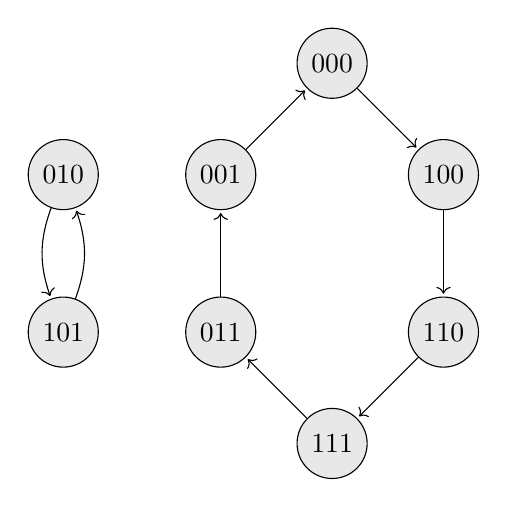
\begin{tikzpicture}[shorten >=1pt,node distance=2cm,auto]
  \tikzstyle{every state}=[fill={rgb:black,1;white,10}]
  \node[state] (zzz) {$000$};
  \node[state] (ozz) [below right of=zzz] {$100$};
  \node[state] (zzo) [below left of=zzz] {$001$};
  \node[state] (ooz) [below of=ozz] {$110$};
  \node[state] (zoo) [below of=zzo] {$011$};
  \node[state] (ooo) [below left of=ooz] {$111$};

  \node[state] (zoz) [left of=zzo] {$010$};
  \node[state] (ozo) [left of=zoo] {$101$};

  \path[->]
  (zoz)  edge [bend right=20] node {} (ozo)
  (ozo)  edge [bend left=-20] node {} (zoz)
  
  (zzz) edge node {} (ozz)
  (ozz) edge node {} (ooz)
  (ooz) edge node {} (ooo)
  (ooo) edge node {} (zoo)
  (zoo) edge node {} (zzo)
  (zzo) edge node {} (zzz);
\end{tikzpicture}
\end{center}
\vspace{1em}
\centerline{Before}

\columnbreak

\begin{center}
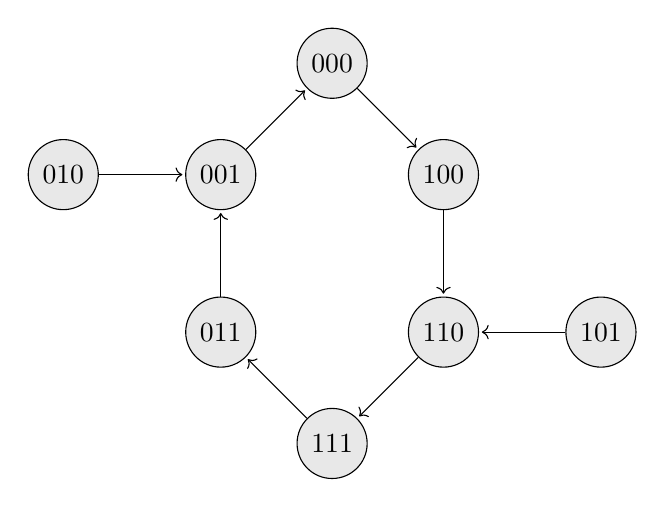
\begin{tikzpicture}[shorten >=1pt,node distance=2cm,auto]
  \tikzstyle{every state}=[fill={rgb:black,1;white,10}]
  \node[state] (zzz) {$000$};
  \node[state] (ozz) [below right of=zzz] {$100$};
  \node[state] (zzo) [below left of=zzz] {$001$};
  \node[state] (ooz) [below of=ozz] {$110$};
  \node[state] (zoo) [below of=zzo] {$011$};
  \node[state] (ooo) [below left of=ooz] {$111$};

  \node[state] (zoz) [left of=zzo] {$010$};
  \node[state] (ozo) [right of=ooz] {$101$};

  \path[->]
  (zoz)  edge node {} (zzo)
  (ozo)  edge node {} (ooz)
  
  (zzz) edge node {} (ozz)
  (ozz) edge node {} (ooz)
  (ooz) edge node {} (ooo)
  (ooo) edge node {} (zoo)
  (zoo) edge node {} (zzo)
  (zzo) edge node {} (zzz);
\end{tikzpicture}
\end{center}
\vspace{1em}
\centerline{After}
\end{multicols}

\subsection*{Q. 4}
\vspace{-5em}
\begin{align*}
S&=x\oplus y\oplus Q\\
C&=xy+Q(x+y)\\
D&=C\\
Q_{t+1}&=D
\end{align*}

\begin{longtable}[c]{ccc|cc|cc}
\hline
x & y & Q & S & C & D & Q(t+1) \\ \hline
\endfirsthead
%
\endhead
%
\hline
\endfoot
%
\endlastfoot
%
0 & 0 & 0 & 0 & 0 & 0 & 0      \\
0 & 0 & 1 & 1 & 0 & 0 & 0      \\
0 & 1 & 0 & 1 & 0 & 0 & 0      \\
0 & 1 & 1 & 0 & 1 & 1 & 1      \\
1 & 0 & 0 & 1 & 0 & 0 & 0      \\
1 & 0 & 1 & 0 & 1 & 1 & 1      \\
1 & 1 & 0 & 0 & 1 & 1 & 1      \\
1 & 1 & 1 & 1 & 1 & 1 & 1      \\ \hline
\end{longtable}
\vspace{1em}
\begin{center}
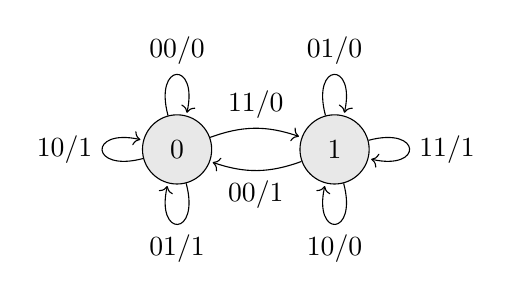
\begin{tikzpicture}[shorten >=1pt,node distance=2cm,auto]
  \tikzstyle{every state}=[fill={rgb:black,1;white,10}]

  \node[state] (o)               {$0$};
  \node[state] (i) [right of=o]  {$1$};

  \path[->]
  (o)  edge [loop above] node {00/0} ( )
       edge [loop below] node {01/1} ( )
       edge [loop left]  node {10/1} ( )
       edge [bend left=20] node {11/0} (i)
  (i)  edge [loop above] node {01/0} ( )
  	   edge [loop below] node {10/0} ( )
  	   edge [loop right] node {11/1} ( )
  	   edge [bend left=20] node {00/1} (o);
\end{tikzpicture}
\end{center}

\begin{center}
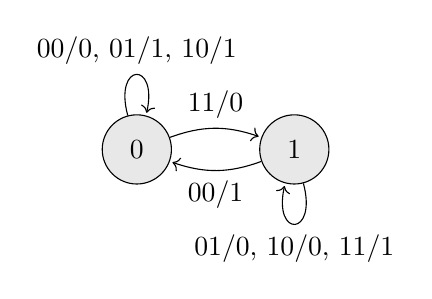
\begin{tikzpicture}[shorten >=1pt,node distance=2cm,auto]
  \tikzstyle{every state}=[fill={rgb:black,1;white,10}]

  \node[state] (o)               {$0$};
  \node[state] (i) [right of=o]  {$1$};

  \path[->]
  (o)  edge [loop above] node {00/0, 01/1, 10/1} ( )
       edge [bend left=20] node {11/0} (i)
  (i)  edge [loop below] node {01/0, 10/0, 11/1} ( )
  	   edge [bend left=20] node {00/1} (o);
\end{tikzpicture}
\end{center}
\centerline{Note that the lines are marked as Input (xy) / Output (S)}

\subsection*{Q. 5}
Knowing that "keeping the least significant bits as such until the first 1, and then complementing all bits", we should shift out the LSB first and let the FSM be in state \emph{a} as shown below. \textit{"Until the first 1"} prompts us to let the condition of stepping into state \emph{b} be meeting the first 1, then FSM should never back to state A, until be reset to ready for another convertion.
\begin{center}
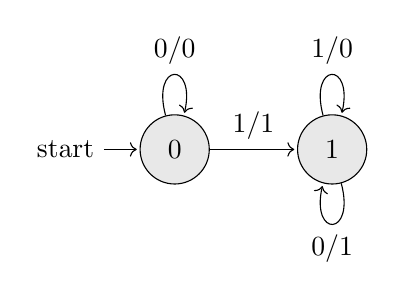
\begin{tikzpicture}[shorten >=1pt,node distance=2cm,auto]
  \tikzstyle{every state}=[fill={rgb:black,1;white,10}]
  \node[state,initial] (a) {$0$};
  \node[state] (b) [right of=a] {$1$};
  \path[->]

  (a) edge [loop above] node {$0/0$} ( )
      edge node {$1/1$} (b)
  (b) edge [loop above] node {$1/0$} ( )
      edge [loop below] node {$0/1$} ( );
\end{tikzpicture}
\end{center}

\begin{longtable}[c]{c|cc|cc}
\hline
\multirow{2}{*}{Present State} & \multicolumn{2}{c|}{Next State} & \multicolumn{2}{c}{Output} \\ \cline{2-5} 
                               & x = 0          & x = 1          & x = 0        & x = 1       \\ \hline
\endfirsthead
%
\endhead
%
0                              & 0              & 1              & 0            & 1           \\
1                              & 1              & 1              & 1            & 0          \\ \hline
\end{longtable}
\vspace{-3em}
\begin{align*}
Q_{t+1}&=x+Q\\
\text{Output}&=x\oplus Q
\end{align*}
\centerline{\includegraphics[width=0.6\textwidth]{fig/q5}}


\par Note that the D-FF should be 0 initially, thus we need a reset signal to help the FSM to step into state \emph{a}.

\section{DIGITAL DESIGN LAB}

\subsection{Task 1}
\begin{lstlisting}[caption={JKFF (Design File)}]
module jkff(
           input clk, rst,
           input j, k,
           output reg q,
           output qn
);
assign qn = ~q;

always @ (posedge clk, negedge rst) begin
    if (!rst) begin
        q <= 0;
    end else begin
        case ({j, k})
            'b00: q <= q;    // keep
            'b11: q <= ~q;   // reverse
            'b10: q <= 1;    // set
            'b01: q <= 0;    // reset
        endcase
    end
end
endmodule
\end{lstlisting}

\begin{lstlisting}[caption={Task 1 - Step 2 (Design File)}]
module task1(
    input clk, rst,
    input x,
    output a, b
);
jkff jk1(clk, rst, ~x, b, a);  // leave qn unwired
jkff jk2(clk, rst, x, ~a, b);  // leave qn unwired
endmodule
\end{lstlisting}

\begin{lstlisting}[caption={JKFF (Testbench)}]
`timescale 1ns/1ps

module jkff_test();
reg clk, rst;
reg j, k;
wire q, qn;

jkff jk(clk, rst, j, k, q, qn);

initial begin
    clk = 0;
    forever #10 clk = ~clk;
end

initial begin
    {rst, j, k} = 'b000;
    #5;  // to demostrate that FF only changes its output at posedge clk
    while ({rst, j, k} < 'b111) begin
        #20 {rst, j, k} = {rst, j, k} + 'b1;
    end
    #10 $finish();
end
endmodule
\end{lstlisting}
\begin{lstlisting}[caption={Task 1 - Step 2 (Testbench)}]
`timescale 1ns/1ps

module task1_test();
reg clk, rst;
reg x;
wire a, b;

task1 tsk1(clk, rst, x, a, b);

initial begin
    clk = 0;
    forever #10 clk = ~clk;
end

initial begin
   {clk, rst, x} = 'b000;
   #100 x = 1;
   #100 x = 0;
   #20 $finish(); 
end

initial begin
    #50 rst = ~rst;
end
endmodule
\end{lstlisting}

\centerline{\includegraphics[width=0.8\textwidth]{fig/jkff}}
\par The waveform of JKFF's simulation shows: \ding{172} When the \textbf{rst} is set 0, JKFF always outputs 0 as q and 1 as q\_n, since the rst is low-activated; \ding{173} No matter when do \textbf{J \& K} change, the JKFF only changes its output at \textbf{posedge clk}, as 130 ns shows; \ding{174} When not in the reset mode, the four cases of \{j, k\} can properly set / reset / keep / reverse q.\\~\\

\centerline{\includegraphics[width=0.8\textwidth]{fig/t1q2}}
\par We first demonstrate the reset mode in 0 - 50 ns, then by comparing the waveform and the state diagram we drew in Q. 2, we say the code works correctly: starting from 50 ns, when \{a, b\} is 00, given x = 0 will let it step into state 10, and the left 0 make it loop in state 10. In state 10, x = 1 lets it step into 11, then whatever x is, it steps into 01 in the next palus, after that, it keep switching the state between 00 and 01, unless a zero lets it changed into 10.

\begin{center}
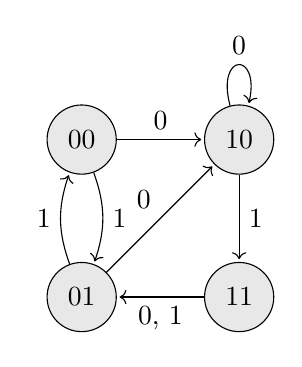
\begin{tikzpicture}[shorten >=1pt,node distance=2cm,auto]
  \tikzstyle{every state}=[fill={rgb:black,1;white,10}]

  \node[state] (zz)               {$00$};
  \node[state] (zo) [below of=zz] {$01$};
  \node[state] (oz) [right of=zz] {$10$};
  \node[state] (oo) [below of=oz] {$11$};

  \path[->]
  (zz)  edge [bend left=20] node {1} (zo)
        edge node {0} (oz)
  (zo)  edge [bend left=20] node {1} (zz)
        edge node {0} (oz)
  (oz)  edge [loop above] node {0} ( )
        edge node {1} (oo)
  (oo)  edge node {0, 1} (zo);
\end{tikzpicture}
\end{center}

\subsection{Task 2}
\begin{lstlisting}[caption={Shifting Register 74195 (Design File)}]
module sr74195(
    input cp, mr_n, pe_n,
    input j, k_n,
    input d3, d2, d1, d0,
    output reg q3, q2, q1, q0,
    output q0_n
);
assign q0_n = ~q0;

always @ (posedge cp, negedge mr_n) begin
    if (!mr_n) begin
        {q3, q2, q1, q0} <= 'b0000;
    end else begin
        if (!pe_n) begin
            {q3, q2, q1, q0} <= {d3, d2, d1, d0};
        end else begin
            case ({j, ~k_n})
                'b00: {q3, q2, q1, q0} <= {q2, q1, q0, q0};
                'b11: {q3, q2, q1, q0} <= {q2, q1, q0, ~q0};
                'b10: {q3, q2, q1, q0} <= {q2, q1, q0, 1'b1};
                'b01: {q3, q2, q1, q0} <= {q2, q1, q0, 1'b0};
            endcase
        end
    end
end
endmodule
\end{lstlisting}

\begin{lstlisting}[caption={Johnson Counter (Design File)}]
module johnson(
    input clk, rst_n,
    output [3:0] qs
);
sr74195 sr(clk, rst_n, 0, 0, 0,
           ~qs[0],qs[3],qs[2],qs[1],
           qs[3], qs[2], qs[1], qs[0]);
endmodule
\end{lstlisting}



\begin{lstlisting}[caption={Shifting Register 74195 (Testbench)}]
`timescale 1ns/1ps

module sr74195_test();
reg cp, mr_n, pe_n;
reg j, k_n;
reg d3, d2, d1, d0;
wire q3, q2, q1, q0, q0_n;

sr74195 sr(cp, mr_n, pe_n, j, k_n,
           d3, d2, d1, d0,
           q3, q2, q1, q0, q0_n);

initial begin
    cp = 0;
    forever #5 cp = ~cp;
end

initial begin
    {j, k_n, mr_n, pe_n} = 4'b0000;  // reseting, enable parallel input
    {d3, d2, d1, d0} = 4'b0101;
    #5 mr_n = 1'b1;  // not reseting
    #10 {d3, d2, d1, d0} = 4'b1010;  // demostrating parallel input
    #10 mr_n = 1'b0;  // master reset
    #10 {mr_n, pe_n} = 2'b11;  // not reseting, disable parallel input

    while ({j, k_n} < 2'b11) begin
        #10 {j, k_n} = {j, k_n} + 1;  // each time, shifting in 2 bits
    end
    #10 $finish();
end

endmodule
\end{lstlisting}

\begin{lstlisting}[caption={Johnson Counter (Testbench)}]
`timescale 1ns/1ps

module johnson_test();
reg clk, rst_n;
wire [3:0] out;

johnson js(clk, rst_n, out);

initial begin
    clk = 0;
    forever #5 clk = ~clk;
end

initial begin
    rst_n = 0;
    #10 rst_n = 1;
    #200 $finish();
end
endmodule
\end{lstlisting}

\centerline{\includegraphics[width=0.6\textwidth]{fig/sr}}
\par This waveform first shows enabling parallel input, then demo the master reset function. After that, disabling the parallel input and start to shifting in digits, using the rule of JKFF.

\vspace{1.5em}
\centerline{\includegraphics[width=0.6\textwidth]{fig/js}}
\par Trivally, this Johnson Counter works as we expected.

\subsection{Task 3}
\begin{lstlisting}[caption={Design File}]
`timescale 1ns/1ps

module freq_div#(parameter N = 1000)(
           input clk,
           input rst,
           output reg clk_out
);
integer counter;
always @(posedge clk, posedge rst) begin
    if (rst) begin
        clk_out <= 0;
        counter <= 0;
    end
    else if (counter == N-1) begin
        clk_out <= ~clk_out;
        counter <= 0;
    end
    else begin
        counter <= counter + 1;
    end
end
endmodule


module seg_tube (
    input clk, mode,  // mode ? CS207 : 2021F
    input rst,
    output reg [7:0] seg_en,
    output reg [7:0] seg_out
);

reg [2:0] now_state;

always @ (posedge clk, posedge rst) begin
    if (rst) now_state <= 0;
    else begin
        if (now_state == 4) now_state <= 0;
        else now_state <= now_state + 1;
    end
end

always @ (now_state) begin
    seg_en = ~(8'b1 << now_state);
    case (now_state)
        0: seg_out = mode ? 8'b1111_1000   // 7
                          : 8'b1000_1110;  // F
        1: seg_out = mode ? 8'b1100_0000   // 0
                          : 8'b1111_1001;  // 1
        2: seg_out =        8'b1010_0100;  // 2
        3: seg_out = mode ? 8'b1001_0010   // S
                          : 8'b1100_0000;  // 0
        4: seg_out = mode ? 8'b1100_0110   // C
                          : 8'b1010_0100;  // 2
        default: seg_out  = 8'b1111_1111;  // DISABLE
    endcase
end
endmodule


module top (
    input clk, rst,
    input mode,
    output [7:0] seg_en, seg_out
);
wire sub_clk;
freq_div#(1000) div(clk, rst, sub_clk);
seg_tube st(sub_clk, mode, rst, seg_en, seg_out);
endmodule
\end{lstlisting}


\begin{lstlisting}[caption={Constraint File}]
set_property IOSTANDARD LVCMOS33 [get_ports {seg_en[7]}]
set_property IOSTANDARD LVCMOS33 [get_ports {seg_en[6]}]
set_property IOSTANDARD LVCMOS33 [get_ports {seg_en[5]}]
set_property IOSTANDARD LVCMOS33 [get_ports {seg_en[4]}]
set_property IOSTANDARD LVCMOS33 [get_ports {seg_en[3]}]
set_property IOSTANDARD LVCMOS33 [get_ports {seg_en[2]}]
set_property IOSTANDARD LVCMOS33 [get_ports {seg_en[1]}]
set_property IOSTANDARD LVCMOS33 [get_ports {seg_en[0]}]
set_property IOSTANDARD LVCMOS33 [get_ports {seg_out[7]}]
set_property IOSTANDARD LVCMOS33 [get_ports {seg_out[6]}]
set_property IOSTANDARD LVCMOS33 [get_ports {seg_out[5]}]
set_property IOSTANDARD LVCMOS33 [get_ports {seg_out[4]}]
set_property IOSTANDARD LVCMOS33 [get_ports {seg_out[3]}]
set_property IOSTANDARD LVCMOS33 [get_ports {seg_out[2]}]
set_property IOSTANDARD LVCMOS33 [get_ports {seg_out[1]}]
set_property IOSTANDARD LVCMOS33 [get_ports {seg_out[0]}]
set_property IOSTANDARD LVCMOS33 [get_ports clk]
set_property IOSTANDARD LVCMOS33 [get_ports mode]
set_property IOSTANDARD LVCMOS33 [get_ports rst]
set_property PACKAGE_PIN Y18 [get_ports clk]
set_property PACKAGE_PIN W4 [get_ports mode]
set_property PACKAGE_PIN S6 [get_ports rst]
set_property PACKAGE_PIN A18 [get_ports {seg_en[7]}]
set_property PACKAGE_PIN A20 [get_ports {seg_en[6]}]
set_property PACKAGE_PIN B20 [get_ports {seg_en[5]}]
set_property PACKAGE_PIN E18 [get_ports {seg_en[4]}]
set_property PACKAGE_PIN F18 [get_ports {seg_en[3]}]
set_property PACKAGE_PIN D19 [get_ports {seg_en[2]}]
set_property PACKAGE_PIN E19 [get_ports {seg_en[1]}]
set_property PACKAGE_PIN C19 [get_ports {seg_en[0]}]
set_property PACKAGE_PIN E13 [get_ports {seg_out[7]}]
set_property PACKAGE_PIN C15 [get_ports {seg_out[6]}]
set_property PACKAGE_PIN C14 [get_ports {seg_out[5]}]
set_property PACKAGE_PIN E17 [get_ports {seg_out[4]}]
set_property PACKAGE_PIN F16 [get_ports {seg_out[3]}]
set_property PACKAGE_PIN F14 [get_ports {seg_out[2]}]
set_property PACKAGE_PIN F13 [get_ports {seg_out[1]}]
set_property PACKAGE_PIN F15 [get_ports {seg_out[0]}]
\end{lstlisting}

\centerline{\includegraphics[width=0.4\textwidth]{fig/cs}\quad \includegraphics[width=0.4\textwidth]{fig/21f}}

\par The above uses the right most switch (W4) to change the contents. When it is switched on, it displays "CS207", while off, displays "2021F".
\end{document}